\documentclass[11pt]{article}

\usepackage{fancyhdr}
\usepackage[margin=1in]{geometry}
\usepackage{xcolor,colortbl}
\usepackage[labelfont=bf,font=small]{caption}


\usepackage[T1]{fontenc}

\usepackage{enumitem}
\usepackage{todonotes}
\usepackage{titlesec}
\usepackage{tabularx}
\usepackage{parskip}
\usepackage{hyperref}
\usepackage{wrapfig}
\titlespacing\section{0pt}{0pt plus 4pt minus 2pt}{0pt plus 2pt minus 2pt}
\titlespacing\subsection{0pt}{12pt plus 4pt minus 2pt}{0pt plus 2pt minus 2pt}
\titlespacing\subsubsection{0pt}{12pt plus 4pt minus 2pt}{0pt plus 2pt minus 2pt}

\definecolor{Gray}{gray}{0.85}
\pagestyle{fancy}
\rfoot{\thepage}
\lfoot{\textbf{Teaching Statement} | D.A. Szafir}
\cfoot{}
\renewcommand{\headrulewidth}{0pt}
\renewcommand{\footrulewidth}{0.5pt}

%opening


\begin{document}
\setlength{\belowcaptionskip}{-10pt}
%\maketitle

\thispagestyle{fancy}

\textbf{\Large Teaching Statement}
{\hspace{220pt}\emph{Danielle Albers Szafir} \vspace{3pt}}
\hrule
%\\
%	{ 
%	\begin{tabularx}{\textwidth}{X X}
%		Assistant Professor & 315 UCB\\ 
%		Department of Information Science & University of Colorado Boulder \\ 
%		College of Media, Communication, \& Information &  Boulder, CO, 80309\\
%		University of Colorado Boulder & danielle.szafir@colorado.edu | 303.492.8532 
%	\end{tabularx}}}
%\hrule

My teaching has largely focused on technologically-oriented courses where students leverage computation to solve real-world problems. In the classroom, I focus on developing a broad understanding of skills necessary to tackle data-oriented problems. My approach to teaching emphasizes hands-on activities and engagement with external stakeholders and real datasets whenever possible. 

\section*{Summary of Accomplishments}

At CU, I have designed and implemented three new courses and served as instructor of record for four courses (one co-taught, two required undergraduate). 246 students completed these courses with a mean instructor rating of 4.5 and a mean course rating of 3.7. These courses have exposed students to real-world data problems through collaboration with eight community stakeholders. I have additionally served as the instructor for 18 independent studies (16 research-oriented and 2 as a computer graphics intensive). 

My first year at CU, I served as part of the founding faculty in the Department of Information Science, where I worked with a team of faculty to develop innovative interdisciplinary curricula at the intersection of computer science, data science, social science and design. We crafted three new degree programs (an Information Science major, minor, and Ph.D.) based on a forward-looking perspective on the discipline. I have continued some of these efforts at part of both the Information Science Graduate Committee and a committee on the computational and quantitative undergraduate course sequences. Additionally, I co-chaired and continue to serve on the Digital Humanities Graduate Certificate Committee which will launch in Fall 2018. 

\section*{Courses Offered}

\textbf{Fall 2016--Computational Reasoning I: }
Co-instructor Steve Voida and I designed the first offering of Computational Reasoning I---the Information Science introductory programming class---for Fall 2017. In this course, we exposed students to the foundations of computing in Python using media manipulation. Built on Georgia Tech's Media Computation course, students learned about variables, lists, conditionals, loops, and functions by programmatically manipulating strings, images, and audio files. In a series of projects, they moved from simple string search and reversal functions to creative image composition by the end of the course. In class, students attended lectures, worked on small-group peer instruction exercises, and participated in live coding exercises and in weekly labs they worked with TAs on smaller lab assignments to enforce skills learned in-class.

This course was a required course for CMCI and a first-time offering in addition to my first large course as instructor of record. Further, the style of the course and mathematical and programmatic thinking required in the course was a significant challenge for many of the students who struggled to understand why they needed a technical course given their career path. While we worked hard to try to make the materials relevant and polled students twice as to how to improve the course and its relevance, we still had some students who did not see the utility of the course itself. These challenges lead to historically lower overall course ratings. However, subjective feedback from the students indicated that they appreciated the engagement with the course and the efforts made by the teaching staff to make the materials accessible. A number of students transfered to Information Science from this first offering after realizing how technology could support their career goals. 

\emph{End-of-Course Enrollment: }134 undergraduate CMCI students\\
\emph{Mean Instructor Rating:} 5.0\\
% (\$174,925)
\emph{Mean Course Rating: 3.7} 

\textbf{Spring 2017, Spring 2018--Information Visualization: } 
This course serves as a Mastery elective for the Department of Information Science and attracts students from all over campus, including Computer Science, Creative Technologies, and Business. In this course, students learn the fundamentals of designing, building, and evaluating information visualization tools, with an emphasis on tools for exploratory data analysis. In class, students attend lecture, participate in reading discussions, and complete hands-on sketch-based activities. Students additionally complete three small team projects building interactive visualization systems using data from local stakeholders and an open-ended final project on a topic of their choosing. 

\begin{wrapfigure}{r}{0.5\textwidth}
	\begin{center}
		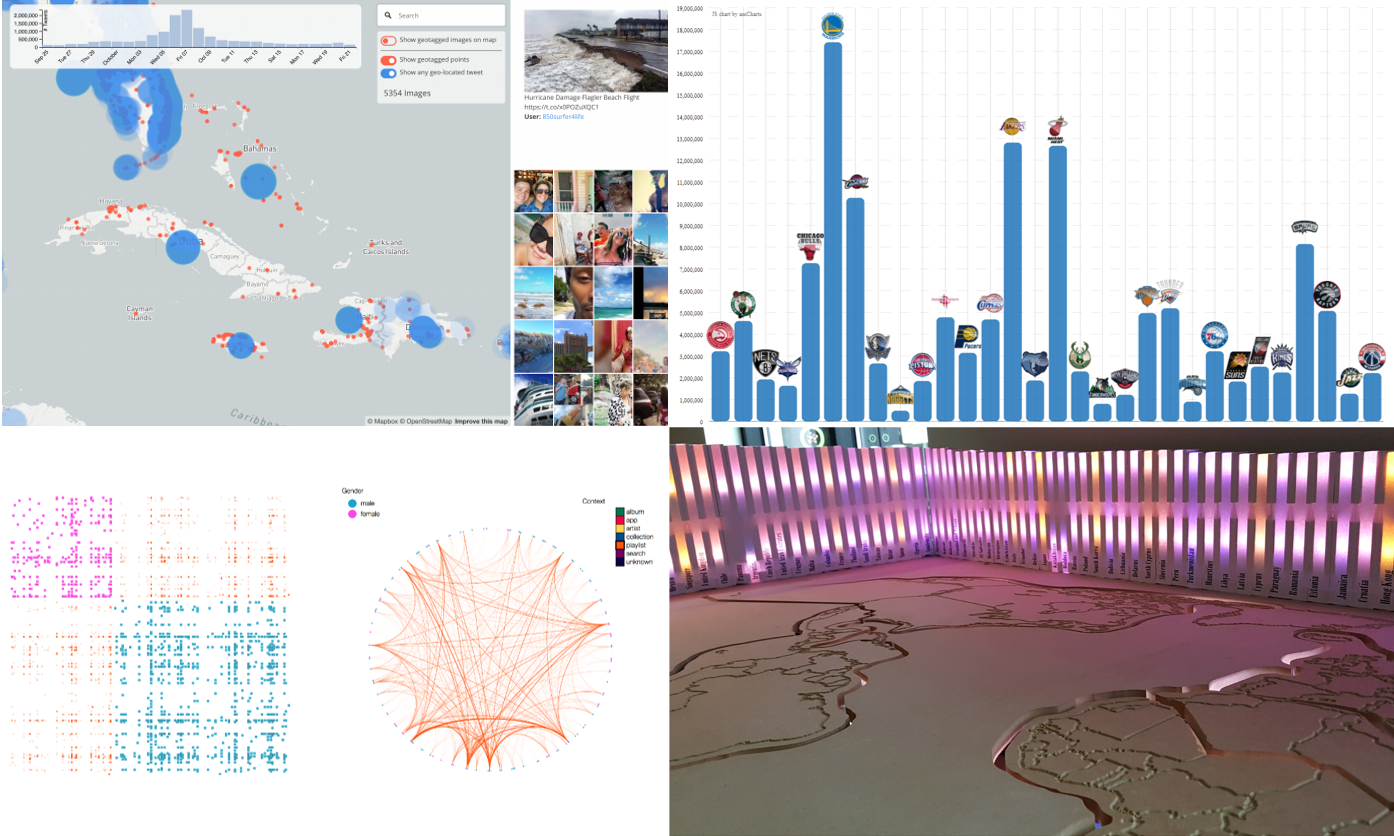
\includegraphics[width=0.48\textwidth]{FlyerImage}
	\end{center}
	\caption{Interactive student projects from INFO 4602/5602 include Twitter image maps, exploring NBA statistics, navigating social networks in Spotify, and interactive physicalizations.}
\end{wrapfigure}

The first offering of this course used consumer data from Zayo, during which students worked alongside Zayo employees to understand the needs of the dataset, presented their solutions at Zayo's Boulder office, and provided \$10k in supplementary funding for the course. At least one student had an interview with the Zayo data team as a result of the project. The second offering used computing demographic data from NCWIT and privacy data from the Knight Foundation, who is currently authoring a blog post featuring some of their favorite student solutions. 

The 2017 offering was a new offering from the Department of Information Science. 
%Note that a smaller offering was made by CSCI in Fall 2016 as a graduate seminar; however, the Information Science offering included undergraduates and a different pedagogical focus, emphasizing technique rather than data domain.  
This course, offered as a joint undergraduate and graduate course, has now been offered two semesters, with the second offering increasing in enrollment by 57.5\%. The biggest challenge in this course has been dealing with the skills gaps between the graduate and undergraduate and computing and design students. Splitting projects into grad-only and undergrad-only teams has significantly aided this challenge (though mid-semester student feedback suggests the concerns are not fully resolved); however, student feedback suggested that more improvement is needed. Future offerings will include more opportunities for physicalization use and a narrower set of platforms to more tightly scope projects.

\emph{End-of-Course Enrollment: }2017--40 students (INFO, CSCI, PSYC); 2018--63 students (INFO, CSCI, BUSM, STCM, MATH, ATLS, IPHY)\\
\emph{Mean Instructor Rating:} 2017--5.3; 2018--5.0\\
\emph{Mean Course Rating:} 2017--4.6; 2018--4.3

\textbf{Fall 2017--Information Exploration: } 
This course serves as a required course for undergraduate Information Science majors. The intention of this course is to scaffold students from skills-oriented courses to domain-oriented courses by providing them with a toolbox for exploratory data analysis, covering the foundations of project management, data collection, machine learning, inferential statistics, visual analytics, and qualitative analysis. Essentially, the course aims to move students from analytics in the small to analytics in the large. During the course, students worked with 17 real-world datasets in a combination of project-based assignments and in-class small-group labs. In class, students attended lecture, participated in regular peer-instruction assignments, participated in reading discussions, and completed an in-class lab every Friday. The course culminated in an open-ended final project where student teams engaged with community stakeholders to solve a data-oriented problem (the CU Independent, Community Foodshare of Colorado, Boulder County Waste Management, the Paul Lab, and the Office of Information Technology). 

\begin{wrapfigure}{l}{0.5\textwidth}
	\begin{center}
		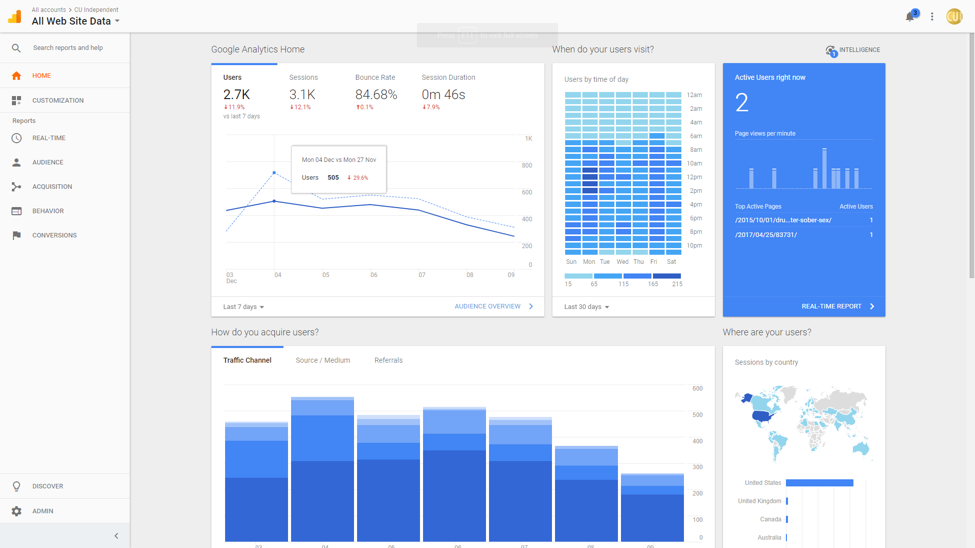
\includegraphics[width=0.48\textwidth]{3401_example}
	\end{center}
	\caption{Student projects engaged real stakeholders through data, such as identifying opportunities for search engine optimization at the CU Independent.}
\end{wrapfigure}

The 2017 offering of this course was a new offering from the Department of Information Science. The course depends heavily on the materials covered in earlier courses---especially INFO 2201 and 2301---for students to comprehend the material. However, the initial offering of the course was designed based on the syllabi for these courses rather than active engagement by 2201 and 2301 instructors, which were both also first time offerings. As a result, there were two significant challenges in the initial delivery: (1) the materials required knowledge that the students did not yet have (and therefore some materials were perceived as too difficult) and (2) the expectations for this course were unclear (students expected another introductory programming course). These issues combined with possible gender issues (students were all male and never attended office hours despite extra offerings around assignments which may have been a by-product of discomfort) led to low FCQ scores. To resolve these issues for the 2018 delivery, we have updated the prerequisite structure to require \emph{both} 2201 and 2301. I have been actively participating in discussions of the INFO Quantitative/Computational Sequence to ensure that Exploration's content aligns appropriately with the prior courses in the sequence. Further, as the in-class lab assignments seemed to significantly assist learning and students requested more in-class programming, I am restructuring the course using a flipped classroom approach, where video lectures will focus on abstract concepts and in-class activities will emphasize how to put these ideas into practice. 

\emph{End-of-Course Enrollment: }2017--9 students\\
\emph{Mean Instructor Rating:} 2017--2.7\\
\emph{Mean Course Rating:} 2017--2.2

\section*{Additional Teaching-Related Activities}

In addition to the above courses, I served as a founding faculty member in the Department of Information Science during which I helped co-design a new major, minor, and Ph.D. curriculum for Information Science. This curriculum blends design, computation, and social aspects of human-data interaction to provide innovative interdisciplinary training for computing-oriented careers.  One of only a handful of undergraduate Information Science programs in the country, our curriculum leverages the unique strengths of our faculty to expose students to diverse skills and problem-solving approaches in order to become conscientious contributors to an increasingly data- and computing-oriented society. Work in this role included program development, course design, and synthesizing a curriculum blending diverse interdisciplinary ideas. During this year, I also attended the Computing Research Association's Early Career Teaching Workshop to prepare professionally for designing and delivering this new material to an intellectually diverse set of undergraduate students. 

Since launching this curriculum in Fall 2016, I continue to participate in curriculum development as part of the undergraduate committee on computational and quantitative reasoning, focusing on how our courses help students develop sufficient statistical and programming literacy to succeed in technical careers. Further, I have actively assisted with graduate course development as a member of the graduate committee, focusing on how to best revise and remain nimble in our graduate requirements in order to support the growing diversity of research areas active in our department. 

At a campus level, I co-chaired a committee to develop a graduate certificate in the Digital Humanities. This certificate focuses on bridging the gap between technical and humanist practices by exposing graduate students to multidisciplinary coursework emphasizing a broad variety of skills. I serve as the representative for and liaison to the technical disciplines. During my time on this committee, we designed a set of certificate requirements based on existing programs focusing on how to achieve more balanced integration of the disciplines, collected letters of support from instructors and chairs of 15 departments, and obtained formal approval for the program starting Fall 2018. 

In addition to this curricular committee work, I have supervised 18 independent studies with undergraduates and masters students from Computer Science, Applied Math, and Creative Technologies. My work in these independent studies has largely focused on small-team endeavors that expose students to visualization and graphics research. So far, these efforts have led to four paper submissions (one conditionally accepted) and several papers underway. I also taught a one-semester Computer Graphics crash course to two independent study students. This course worked through a series of hands-on activities to learn the fundamentals of computer graphics covering materials inclusive of and extending the current graphics course offerings using a suite of tools and techniques better suited to modern graphics research. Based on the outcomes of this activity, I intend to develop these materials into a formal Mastery course offered through Information Science. 

%Curriculum committees: comp/quant sequence, graduate course restructuring, 

%Student mentorship, including graduate capstone, 16 semesters independent study 

I have given 13 guest lectures at CU and one in the Library and Information Science program at the University of Denver. These lectures covered concepts in visualization, visual communication, computer graphics, and interactive systems engineering for both technical fields (e.g., ATLAS, Information Science, and Computer Science) as well as Museum Studies, where students have a growing interest in engaging technologies to enhance the pedagogical aims of their exhibits. 

%Guest lectures (13 at CU and 1 at DU), graphics and big data

\section*{Current Teaching Trajectory}

In the classroom, I aim to provide students with real-world engagement with data and stakeholders to help them develop relevant technical, communication, and project management skills. Since starting at CU in 2015, I have served as instructor of record for four courses (246 students completing) in addition to significant engagement with students through independent study and guest lectures. In these courses, students have actively engaged with data from eight different organizations and develop skills in programming, statistical analysis, empirical evaluation, project management, and user-centered design.

My efforts to date have largely focused on course design (two required courses and one combined graduate/undergraduate elective). In the process of designing these courses, my aims have mostly been to support conceptual understanding through in-class sketching, small peer-instruction exercises, and similar hands-on activities. My near-term goals are to focus more on refining the classroom delivery of this work. The skills in these courses require not only conceptual understanding but foundational technical skills to implement and execute. Requests for this have come out strongly in the feedback for the most recent iteration of INFO 4602/5602, where students requested a tighter coupling of readings, projects, and lectures. In addition to the specific course plans mentioned above, I plan to revise the current curricula to focus more heavily on implementation and designing activities to help students make the larger step of translating concept into practice. 


\pagebreak
\setcounter{page}{1}


\end{document}
